% !TEX root = ../proposal.tex
%
\chapter{Introduction}
\label{sec:intro}

Best practices in software development changed dramatically since its origins in the 1950's~\cite{boehm2006view}.
Software engineering in most of the 20th century was largely based on careful planning and specification and therefore rather slow-paced and inflexible.
Since twenty years, however, these plan-driven development methods have been frustrating many people because the influencing circumstances change more and more rapidly, not least due to the growing importance of the internet~\cite{Williams2003}.
A result of this rapid change of the environment is that product features, which were perfectly valid at the time of their envisioning, became outdated, irrelevant or otherwise undesirable while the feature was still being planned or implemented -- not to mention features that are in fact not desired by the customers in the first place.
This insight is often not gained until the feature is shipped to the customer.
As a consequence, short release cycles and fast customer feedback have steadily been growing in importance.
These values are emphasized in \acf{CSE}~\cite{Bosch2014}, which adopts and extends the principles from \emph{DevOps} and agile software development~\cite{Fitzgerald2017,fowler2001agile}.

Adopting the core premises of \ac{CSE} is considered to be a gradual process, which is represented by the \emph{Stairway to Heaven}~\cite{Olsson2012} (see~\cref{fig:stairway}).
Starting from classical software development, the next step is agile software development.
This step is followed by continuous integration and deployment, respectively. 
The last step in the Stairway to Heaven is "Research \& Development as an Innovation System".
This means that the continuity gained in the previous steps is used for frequently deploying changes to the customers.
These changes are then assessed by analyzing user feedback data which was previously gathered using active or passive methods.
While active user feedback, e.g. in form of surveys, can yield useful qualitative observations about the product, the fact that the user has to actively take time for giving their feedback is often problematic.
Passive user feedback avoids this problem by automatically collecting feedback while the user works with the system; an example for this is measuring the time a user needs to perform certain actions in the software.
An \emph{evolutionary system} as described here allows for quicker responses to market changes and more accurate estimation of customer needs.

\begin{figure}[htb]
        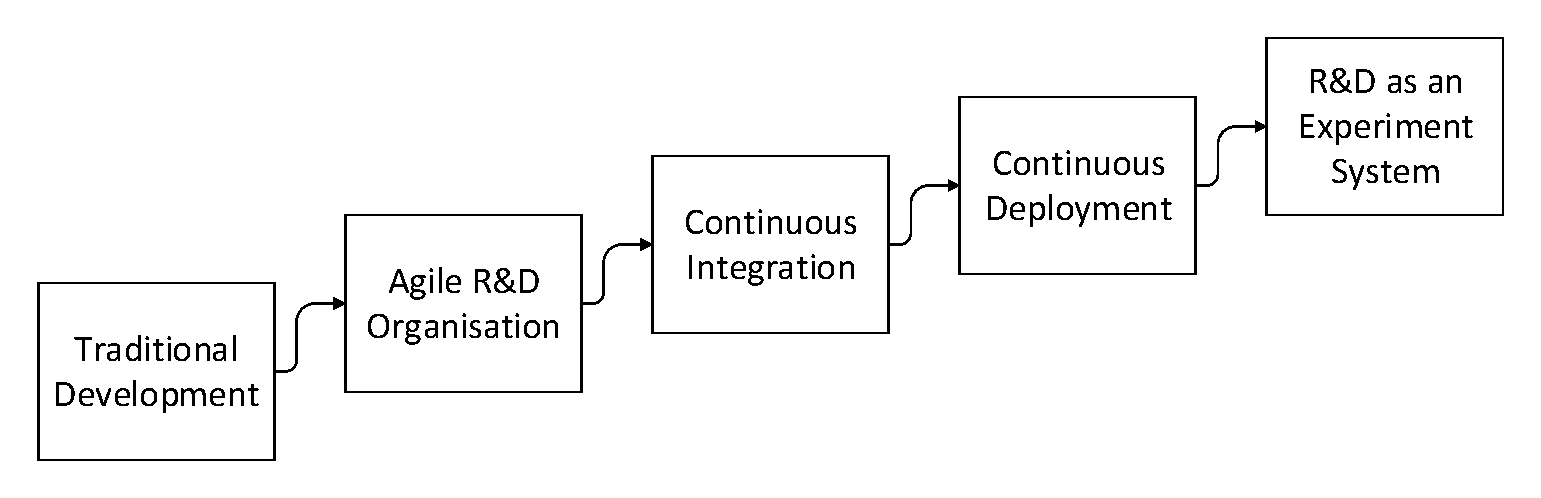
\includegraphics[width=\textwidth]{gfx/stairway}
        \caption{The "stairway to heaven" evolutionary model; adapted from~\cite{Olsson2012}.}
        \label{fig:stairway}
\end{figure}

%\cite{Bosch2014}

%The results of such an experiment are then used for deciding wether the feature should become a part of the final product.
%Thus, the goal in this case is to increase the effectiveness of developing a software product by implementing the \emph{right} features.
%Experiments are also used in order to compare different implementations of the same feature, thus improving the quality of an existing feature.
%This approach is contrary to the more classical software development methods, in which the stakeholders make certain assumptions which result in the envisioning of a feature, with feedback by a customer or stakeholder being given only much later in the development process~\cite{Bosch2012}.

%The core premise in innovation experiment systems is the continuous implementation and validation of assumptions about envisioned features via experiments in short sprints~\cite{Bosch2014}.
%The results of such an experiment are then used for deciding wether the feature should become a part of the final product.
%Thus, the goal in this case is to increase the effectiveness of developing a software product by implementing the \emph{right} features.
%Experiments are also used in order to compare different implementations of the same feature, thus improving the quality of an existing feature.
%This approach is contrary to the more classical software development methods, in which the stakeholders make certain assumptions which result in the envisioning of a feature, with feedback by a customer or stakeholder being given only much later in the development process~\cite{Bosch2012}.

The agile and continuous work methods in \ac{CSE} come with several implications for the system architecture and the company culture~\cite{Lindgren2015,Olsson2012}.
In particular, monolithic software systems are considered too cumbersome and slow to change; instead, small services that communicate with each other through a well defined but lightweight API are recommended.
\citet{ford2017building} argue that such distributed systems work well with the \emph{Parallel Model} concept introduced by \citet{WEB:Fowler:2005-2}.
The rationale is that using Parallel Model, services can work with their own specialized read model without interfering with or complicating the overall application state.
In order to make use of Parallel Model, it is recommended that the system also uses \emph{Event Sourcing}~\cite{WEB:Fowler:2005,WEB:Fowler:2005-2}.
Event sourcing is a storage solution in which data is stored in the form of immutable event objects representing actions on business objects; in combination, all these events represent the application state.
The most obvious advantage of this approach is that the event log represents a complete log of all transactions.
More importantly, however, this also allows for the execution of temporal queries which compute the application state at any given point in time, and the ability to replay events, possibly after modifying the application state at a certain point in time.
A consequence of event replayability is that events can be received in any given sequence, which otherwise is a common problem in asynchronous systems.

This thesis aims at taking a more holistic approach to the innovation system concept from \ac{CSE} by designing and implementing a system that allows for easy collection of passive user feedback (\cref{sec:objectives} describes the objectives in more detail).
The result will be a set of interacting services which provide the ability to collect, aggregate and analyze passive user feedback in order to facilitate innovation in the research and development process.
It is anticipated that this system will profit from the usage of even sourcing, but this has to be further investigated in the thesis.
The resulting system can be adopted by individuals and companies in the software industry who want to fully embrace \ac{CSE} and thus take the last step in the Stairway to Heaven.
